\documentclass{beamer}
\usepackage{color, amsmath, comment, subfigure}
\usepackage{url}

\usepackage{hyperref}
\hypersetup{
    colorlinks=true,
    linkcolor=blue,
    filecolor=magenta,      
    urlcolor=cyan,
}

%%%%%%%%%%%%%%%%%%%%%%%%%%
\title[]{Pre-read for Tuesday, Sept 8: Predicting geopolitical events, part 2}
\author[]{Matthew J. Salganik}
\institute[]{COS 597E/SOC 555 Limits to prediction}
\date[]{Fall 2020, Princeton University}

\begin{document}
%%%%%%%%%%%%%%%%%%%%%%%%%%%
\frame{\titlepage}
%%%%%%%%%%%%%%%%%%%%%%%%%%%
\begin{frame}
\frametitle{}

\begin{center}
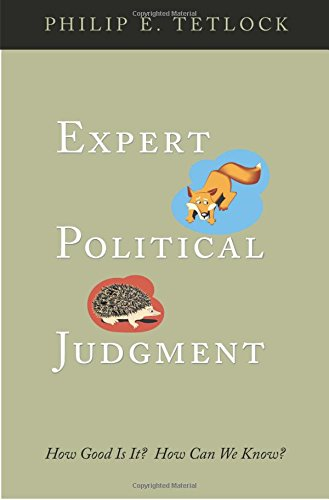
\includegraphics[height=0.7\textheight]{figures/tetlock_expert_2005_cover}
\end{center}

\vfill
20 years in the making

\end{frame}
%%%%%%%%%%%%%%%%%%%%%%%%%%%
\begin{frame}

\begin{center}
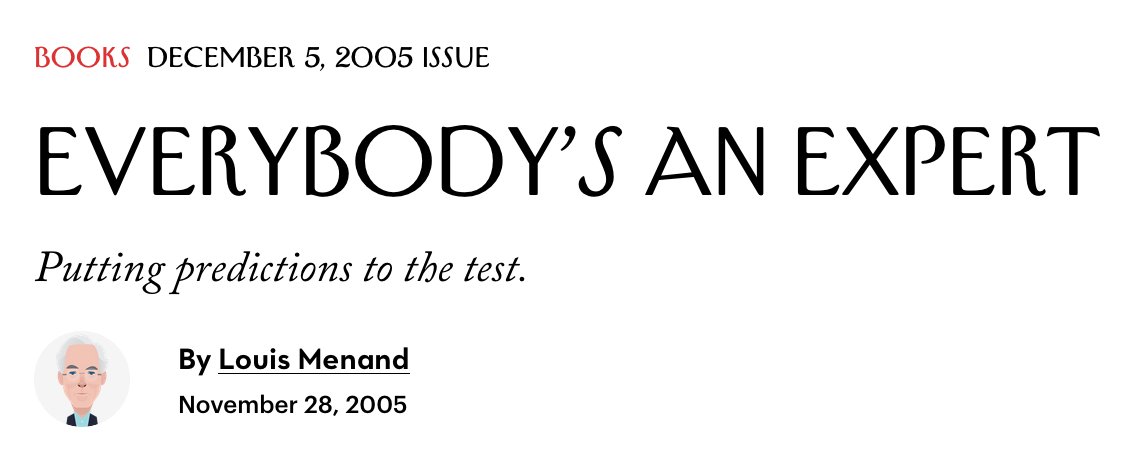
\includegraphics[width=0.7\textheight]{figures/menand_everybodys_2005_title}
\end{center}

\vfill
\url{https://www.newyorker.com/magazine/2005/12/05/everybodys-an-expert}

\end{frame}
%%%%%%%%%%%%%%%%%%%%%%%%%%%
\begin{frame}

\begin{center}
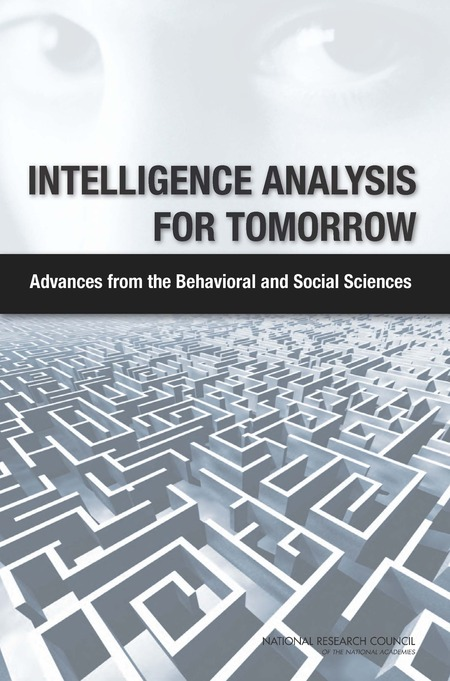
\includegraphics[height=0.7\textheight]{figures/nas_intellegence_2011_cover}
\end{center}

\vfill
\url{https://doi.org/10.17226/13040}

\end{frame}
%%%%%%%%%%%%%%%%%%%%%%%%%%%
\begin{frame}

\begin{center}

\includegraphics[width=0.7\textwidth]{figures/mandel_accuracy_2014_title}
\end{center}

\vfill
\url{https://doi.org/10.1073/pnas.1406138111}

\end{frame}
%%%%%%%%%%%%%%%%%%%%%%%%%%%
\begin{frame}

\begin{center}
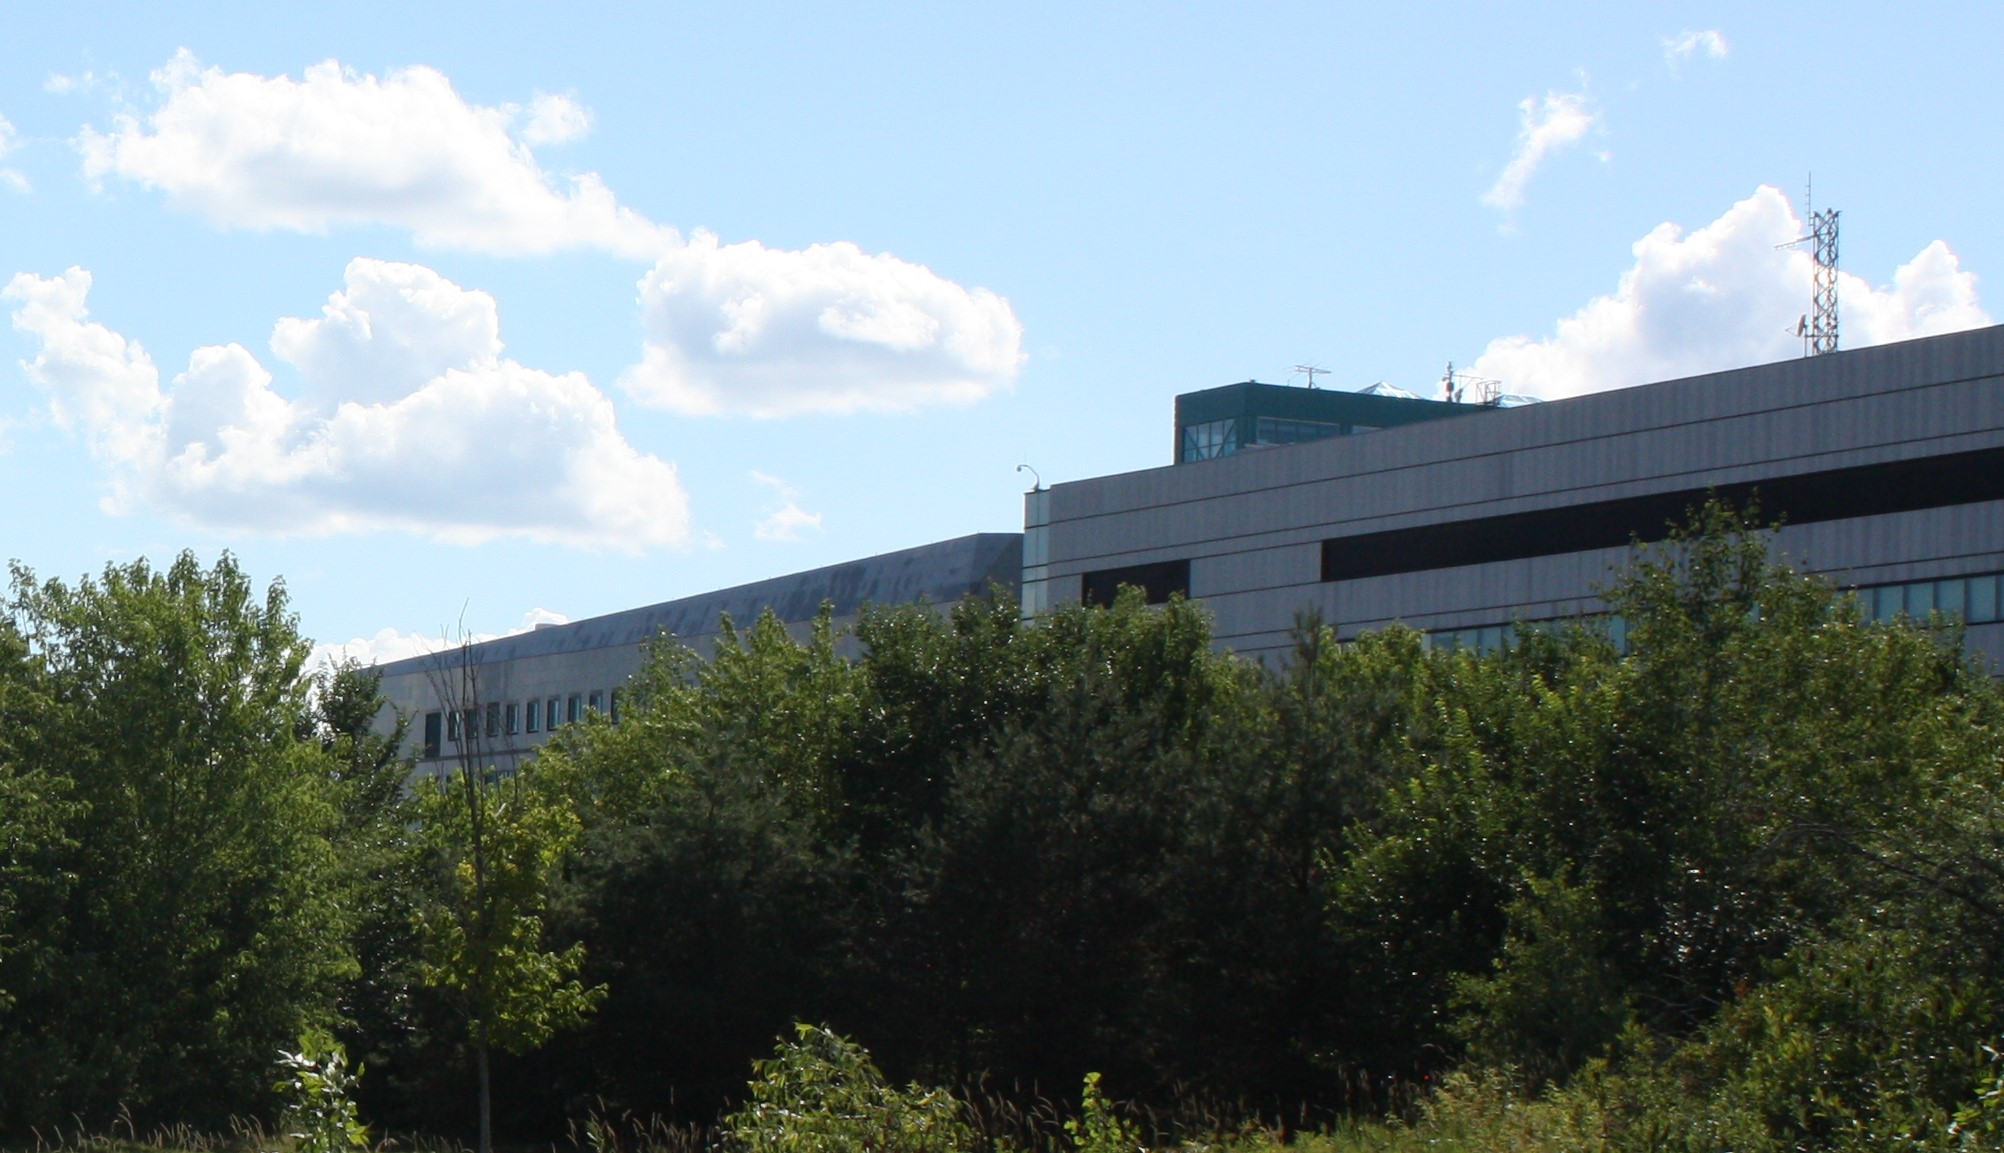
\includegraphics[width=0.7\textwidth]{figures/CSIS_Ottawa_Building_Ogilvie_Canadian_Security_Intelligence_Service_(50182903412)}
\end{center}

\vfill
Intelligence Assessment Secretariat, part of the Canadian Security Intelligence Service
\end{frame}
%%%%%%%%%%%%%%%%%%%%%%%%%%
\begin{frame}

Predictions embedded in reports
\begin{itemize}
\item ``The intense distrust that exists between Country X and Country Y is almost certain [9/10] to prevent the current relationship of convenience from evolving into a stronger alliance.''
\item ``It is very unlikely [1/10] that either of these countries will make a strategic decision to launch an offensive in the coming six months.''
\end{itemize}

\end{frame}
%%%%%%%%%%%%%%%%%%%%%%%%%%%
\begin{frame}

\begin{itemize}
\item How do their predictions compare to the ones by Tetlock's experts?
\pause
\item What variation is there in performance for different types of predictors or outcomes?
\end{itemize}

\end{frame}
%%%%%%%%%%%%%%%%%%%%%%%%%%%
\begin{frame}

Reading notes:
\begin{itemize}
\item Tetlock (2005): roughly 15\% of cases had ambiguous outcomes (p 296), Mandel and Barnes (2014): 20\% of cases had ambiguous outcomes (p 10987)
\pause
\item Who picks tasks?  It seems like analysts pick what they forecast (somewhat)
\pause
\item Hard or easy are coded by experts after the fact
\end{itemize}

\end{frame}
%%%%%%%%%%%%%%%%%%%%%%%%%%%
\begin{frame}

From SI:\\
Low/moderate difficulty included judgments under most or all of the following conditions: \\
(i) availability of a substantial and credible information base, \\
(ii) involving a limited number of factors and/or largely a straight-line continuation of current trends, \\
(iii) little influence of irrational or unpredictable behavior, and \\
(iv) generally involving a short time horizon (several months).\\

Moderate/high difficulty included judgments affected by some of the following conditions: \\
(i) a limited and unreliable information base, \\
(ii) involving a wide range of complicated factors with multiple potential outcomes, \\
(iii) high likelihood of unpredictable behavior, and \\
(iv) involving a longer time horizon (a year or more).

There were 675 easier forecasts and 839 harder forecasts. Providing some indication of reliability, there was less outcome variance in the easier set (VI = 0.19) than in the harder set (VI = 0.25). (But no measure of inter-coder reliability).

\end{frame}
%%%%%%%%%%%%%%%%%%%%%%%%%
\begin{frame}

\begin{center}

\includegraphics[width=0.7\textwidth]{figures/tetlock_judging_2014_title}
\end{center}

\vfill
\url{https://doi.org/10.1073/pnas.1412524111}

\end{frame}
%%%%%%%%%%%%%%%%%%%%%%%%%%
\begin{frame}

Reading notes
\begin{itemize}
\item How do they explain any difference in findings between Mandel and Barnes and Teltock (1995) and Meller and Tetlock (what comes after Tetlock 1995)?
\item What does this mean for our ability to learn anything from an empirical study like this?
\end{itemize}

\end{frame}
%%%%%%%%%%%%%%%%%%%%%%%%%%
\begin{frame}

\begin{center}
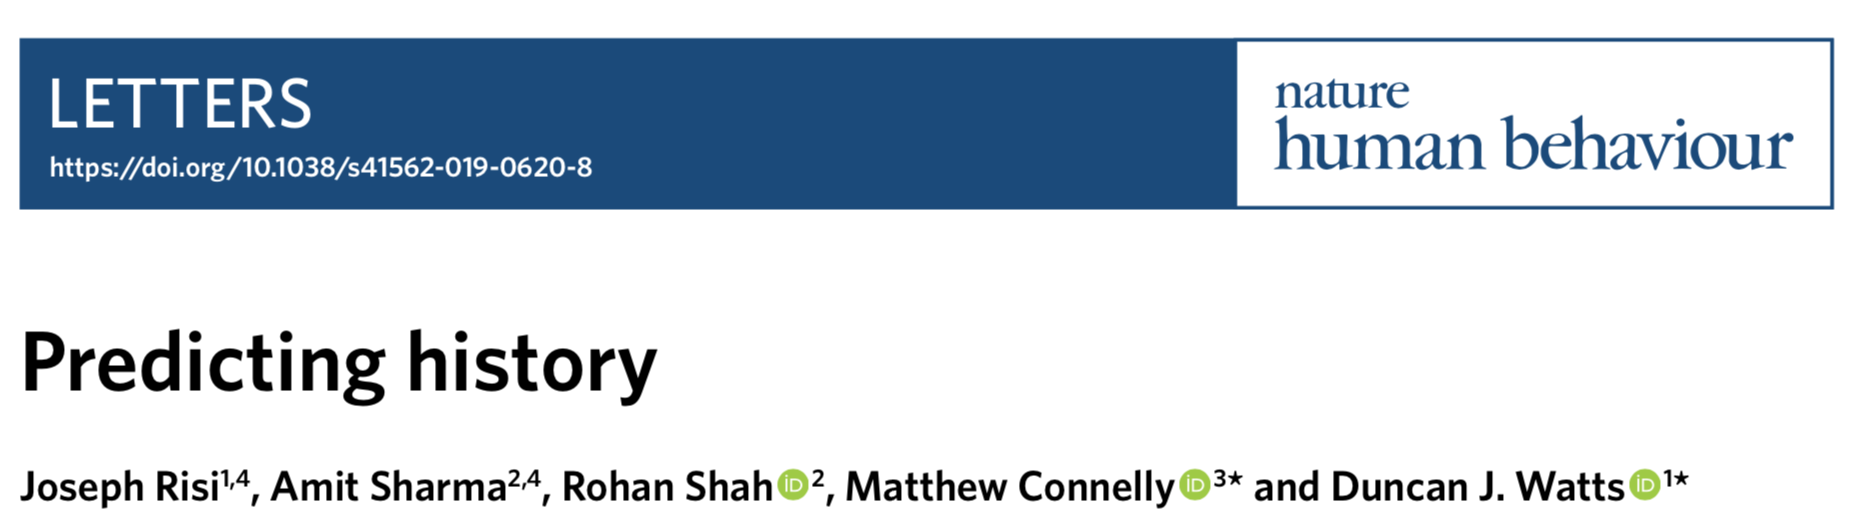
\includegraphics[width=0.7\textwidth]{figures/risi_predicting_2019_title}
\end{center}

\vfill
\url{https://doi.org/10.1038/s41562-019-0620-8}

\end{frame}
%%%%%%%%%%%%%%%%%%%%%%%%%%
\begin{frame}

Danto

\end{frame}
%%%%%%%%%%%%%%%%%%%%%%%%
\begin{frame}

Cables

\end{frame}
%%%%%%%%%%%%%%%%%%%%%%%%%
\begin{frame}

\begin{itemize}
\item How accurately can the perceived contemporaneous impression of importance judgements predict subsequent judgement by historians?
\item How well can an ML model training on the cables predict subsequent judgement by historians?
\item What do the errors of the humans and the algorithms teach us?
\end{itemize}

\end{frame}
%%%%%%%%%%%%%%%%%%%%%%%%%
\begin{frame}

What to read next:
\begin{itemize}
\item ``Bobby W.'' (2019) \href{https://www.cia.gov/library/center-for-the-study-of-intelligence/csi-publications/csi-studies/studies/vol-63-no-4/Limits-of-Prediction.html}{The Limits of Prediction---or How I Learned to Stop Worrying About Black Swans and Love Analysis} ``The key struggle for intelligence analysts is that they are made to produce and what their consumers think they can produce are often two different things.''
\item Doran (1999) \href{https://www.jstor.org/stable/3186379}{Why Forecasts Fail: The Limits and Potential of Forecasting in International Relations and Economics}
\item What to read next from last class
\end{itemize}

\end{frame}
%%%%%%%%%%%%%%%%%%%%%%%%%%%

\end{document}
